\documentclass[11pt,letterpaper]{article}
\usepackage[margin=0.65in]{geometry}
\usepackage{amsmath,amssymb}
\usepackage[T1]{fontenc}
\usepackage{lmodern}
\usepackage{graphicx}
\usepackage{tikz}
\usetikzlibrary{arrows.meta}
\usepackage[hidelinks]{hyperref}
\pagestyle{empty}
\setlength{\parindent}{0pt}
\setlength{\parskip}{3pt}
\setlength{\jot}{1pt}
\setlength{\abovedisplayskip}{5pt}
\setlength{\belowdisplayskip}{5pt}
\begin{document}
\begin{center}
{\large\bfseries Downforce Optimization of an Airfoil in Ground Effect}\\[3pt]
Ling Xiao and Michael Zhang \quad Group 7 \quad AER 588 \quad October 16, 2026
\end{center}
\vspace{-7pt}

\textbf{Application and model.}
We will maximize downforce on a racing-car front-wing section under drag and geometric limits. The initial NACA 0012 has reference chord $c=0.50$\,m, clearance $0.05$\,m, and incidence $-3^\circ$; incidence will vary. Speed is $200$\,km/h ($M\approx0.163$, $Re_c\approx1.90\times10^6$). The open-source \href{https://mdolab-mach-aero.readthedocs-hosted.com/}{MACH-Aero framework} provides ADflow steady RANS on a quasi-2D overset O-grid and background grid. We plan a moving no-slip ground, $\boldsymbol{U}_{\rm wall}=(U_\infty,0,0)$, excluding finite-span and vehicle effects.

\textbf{Model evaluation.}
Inputs are FFD shape, incidence, and operating conditions; outputs are $C_L$, $C_D$, pressure, thickness, and clearance. A preliminary 88,548-cell slip-ground solve took 150\,s on four MPI processes; moving-wall and adjoint costs are unmeasured. We will use pyGeo FFD, IDWarp mesh deformation, and ADflow discrete-adjoint derivatives, and perform a grid-independence study.

\textbf{Optimization problem.}
Let $x=(d,\alpha)$ contain independent FFD displacements and incidence; $n$ depends on FFD resolution and coupling. With upward-positive lift and flow state $u(x)$,
\[
\begin{aligned}
\text{minimize}\quad & f(x)=C_L(x,u(x)) \\
\text{by varying}\quad & x=(d,\alpha)\in\mathbb R^n \\
\text{subject to}\quad & C_D(x,u(x))/C_{D,\max}-1\le0, \\
& 1-t_j(x)/t_{\min,j}\le0,\quad j=1,\ldots,N_t, \\
& X_{\min}-X_k(x)\le0,\quad X_k(x)-X_{\max}\le0, \\
& h_{\min}-Y_k(x)\le0,\quad Y_k(x)-h_{\min}-H\le0, \\
& r(u(x),x)=0.
\end{aligned}
\]
Here $r=0$ denotes RANS; the box inequalities apply to all $N_s$ surface points $(X_k,Y_k)$. Initial limits are $h_{\min}=0.05$\,m, $H=0.15$\,m, $[X_{\min},X_{\max}]=[0,c]$, and $t_{\min,j}=0.5t_{j,0}$ at ten interior chord stations. Subscript 0 denotes the baseline; initially $C_{D,\max}=C_{D,0}$ for the moving-ground case. Box containment and minimum thickness are the only geometric constraints. This is a continuous, constrained, nonconvex, PDE-constrained nonlinear program, solved in reduced space.

\textbf{Software and expected learning.}
We will compare IPOPT (interior point) and SLSQP (SQP) through pyOptSparse on P1--P2. A trade study will quantify the downforce gained by relaxing the drag limit and, as stretch goals, varying clearance and box dimensions. We will identify active constraints and use pressure distributions to distinguish geometric limits from flow separation. Comparing starting shapes will reveal sensitivity to local optima and show whether added design freedom produces useful aerodynamic gains.

\vspace{4pt}
\noindent
\begin{minipage}[t]{0.55\linewidth}
\vspace{0pt}
\textbf{Project goals / problem sequence}
\par\vspace{4pt}
\setlength{\tabcolsep}{3pt}
\renewcommand{\arraystretch}{1.02}
\begin{tabular}{@{}l p{0.85\linewidth}@{}}
\hline
Stage & Investigation / deliverable \\
\hline
P0 & Baseline, $h/c$ sweep, grid independence. \\
P1 & Incidence/ride height; contours, optimizer paths. \\
\textbf{P2} & \textbf{Minimum: single-element shape and incidence optimization.} \\
P3 & Drag-limit sweep; other starting shapes. \\
P4 & Vary box height, length, and clearance. \\
P5 & Main element plus flap. \\
P6 & Wake pressure loss as second objective. \\
P7 & Compare one, two, and three elements. \\
\hline
\end{tabular}
\par\vspace{4pt}
P3--P7 are stretch goals.
\end{minipage}\hfill
\begin{minipage}[t]{0.43\linewidth}
\vspace{0pt}
\centering
% Compact Option B: stacked sections make use of the available column height.
\IfFileExists{graphics/option_b_compact.png}{%
\includegraphics[width=\linewidth]{graphics/option_b_compact.png}%
}{%
\resizebox{\linewidth}{!}{%
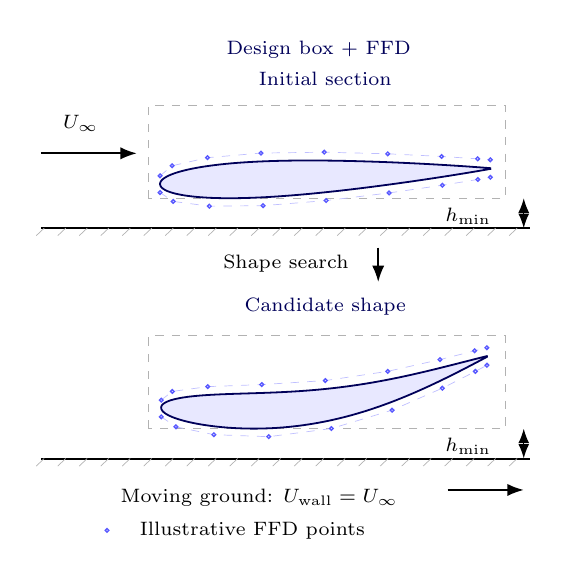
\begin{tikzpicture}[x=4.2cm,y=3.8cm,>=Latex,font=\scriptsize]
\path[use as bounding box] (-.40,-1.07) rectangle (1.16,.67);
\draw[gray!60,dashed] (-.035,0.100) rectangle (1.045,0.410);
\node[above,text=blue!35!black] at (.5,0.445) {Initial section};
\filldraw[fill=blue!9,draw=blue!35!black,line width=.65pt] (0.00034,0.14685) -- (0.00050,0.15008) -- (0.00175,0.15436) -- (0.00346,0.15754) -- (0.00676,0.16176) -- (0.01000,0.16489) -- (0.01534,0.16902) -- (0.02009,0.17207) -- (0.02741,0.17608) -- (0.03364,0.17904) -- (0.04290,0.18290) -- (0.05056,0.18573) -- (0.06169,0.18940) -- (0.07073,0.19207) -- (0.08366,0.19551) -- (0.09400,0.19800) -- (0.10863,0.20117) -- (0.12021,0.20344) -- (0.13644,0.20632) -- (0.14917,0.20836) -- (0.16688,0.21091) -- (0.18068,0.21270) -- (0.19974,0.21491) -- (0.21450,0.21643) -- (0.23477,0.21828) -- (0.25039,0.21953) -- (0.27173,0.22103) -- (0.28809,0.22201) -- (0.31035,0.22315) -- (0.32733,0.22388) -- (0.35034,0.22468) -- (0.36783,0.22516) -- (0.39141,0.22565) -- (0.40928,0.22590) -- (0.43328,0.22609) -- (0.45139,0.22613) -- (0.47563,0.22606) -- (0.49385,0.22592) -- (0.51815,0.22561) -- (0.53635,0.22530) -- (0.56054,0.22479) -- (0.57859,0.22434) -- (0.60249,0.22366) -- (0.62025,0.22309) -- (0.64369,0.22227) -- (0.66104,0.22161) -- (0.68384,0.22067) -- (0.70066,0.21993) -- (0.72266,0.21890) -- (0.73882,0.21811) -- (0.75986,0.21702) -- (0.77525,0.21619) -- (0.79518,0.21507) -- (0.80967,0.21422) -- (0.82835,0.21308) -- (0.84185,0.21223) -- (0.85913,0.21111) -- (0.87154,0.21028) -- (0.88731,0.20919) -- (0.89854,0.20839) -- (0.91268,0.20737) -- (0.92264,0.20663) -- (0.93505,0.20568) -- (0.94368,0.20501) -- (0.95426,0.20417) -- (0.96150,0.20359) -- (0.97018,0.20288) -- (0.97596,0.20240) -- (0.98268,0.20184) -- (0.98697,0.20147) -- (0.99167,0.20107) -- (0.99444,0.20083) -- (0.99709,0.20060) -- (0.99831,0.20049) -- (0.99891,0.20044) -- (0.99904,0.19793) -- (0.99845,0.19781) -- (0.99725,0.19758) -- (0.99463,0.19707) -- (0.99191,0.19655) -- (0.98727,0.19565) -- (0.98304,0.19484) -- (0.97642,0.19358) -- (0.97072,0.19250) -- (0.96216,0.19089) -- (0.95503,0.18955) -- (0.94459,0.18761) -- (0.93608,0.18604) -- (0.92384,0.18381) -- (0.91401,0.18203) -- (0.90005,0.17953) -- (0.88897,0.17756) -- (0.87340,0.17483) -- (0.86115,0.17271) -- (0.84407,0.16978) -- (0.83074,0.16753) -- (0.81228,0.16445) -- (0.79795,0.16209) -- (0.77825,0.15888) -- (0.76304,0.15645) -- (0.74222,0.15317) -- (0.72624,0.15069) -- (0.70446,0.14737) -- (0.68782,0.14488) -- (0.66524,0.14156) -- (0.64805,0.13909) -- (0.62483,0.13582) -- (0.60722,0.13340) -- (0.58352,0.13022) -- (0.56562,0.12789) -- (0.54162,0.12485) -- (0.52355,0.12265) -- (0.49941,0.11980) -- (0.48130,0.11775) -- (0.45720,0.11515) -- (0.43919,0.11329) -- (0.41530,0.11098) -- (0.39751,0.10936) -- (0.37400,0.10738) -- (0.35656,0.10603) -- (0.33359,0.10442) -- (0.31662,0.10337) -- (0.29437,0.10218) -- (0.27800,0.10145) -- (0.25662,0.10070) -- (0.24095,0.10031) -- (0.22060,0.10004) -- (0.20576,0.10001) -- (0.18658,0.10021) -- (0.17266,0.10054) -- (0.15479,0.10123) -- (0.14191,0.10193) -- (0.12547,0.10309) -- (0.11372,0.10414) -- (0.09883,0.10577) -- (0.08829,0.10716) -- (0.07507,0.10923) -- (0.06580,0.11095) -- (0.05435,0.11343) -- (0.04644,0.11544) -- (0.03682,0.11831) -- (0.03032,0.12060) -- (0.02262,0.12383) -- (0.01757,0.12637) -- (0.01184,0.12992) -- (0.00829,0.13269) -- (0.00456,0.13654) -- (0.00253,0.13953) -- (0.00084,0.14365) -- (0.00034,0.14685) -- cycle;
\draw[blue!25,dashed,line width=.25pt] (0.00034,0.17485) -- (0.03671,0.20838) -- (0.14382,0.23552) -- (0.30544,0.25092) -- (0.49689,0.25388) -- (0.68877,0.24846) -- (0.85167,0.23960) -- (0.96062,0.23166) -- (0.99891,0.22844);
\filldraw[fill=white,draw=blue!65,line width=.5pt] (0.00034,0.17485) circle[radius=.65pt];
\filldraw[fill=white,draw=blue!65,line width=.5pt] (0.03671,0.20838) circle[radius=.65pt];
\filldraw[fill=white,draw=blue!65,line width=.5pt] (0.14382,0.23552) circle[radius=.65pt];
\filldraw[fill=white,draw=blue!65,line width=.5pt] (0.30544,0.25092) circle[radius=.65pt];
\filldraw[fill=white,draw=blue!65,line width=.5pt] (0.49689,0.25388) circle[radius=.65pt];
\filldraw[fill=white,draw=blue!65,line width=.5pt] (0.68877,0.24846) circle[radius=.65pt];
\filldraw[fill=white,draw=blue!65,line width=.5pt] (0.85167,0.23960) circle[radius=.65pt];
\filldraw[fill=white,draw=blue!65,line width=.5pt] (0.96062,0.23166) circle[radius=.65pt];
\filldraw[fill=white,draw=blue!65,line width=.5pt] (0.99891,0.22844) circle[radius=.65pt];
\draw[blue!25,dashed,line width=.25pt] (0.00034,0.11885) -- (0.04001,0.08931) -- (0.14937,0.07350) -- (0.31172,0.07509) -- (0.50243,0.09215) -- (0.69270,0.11761) -- (0.85377,0.14344) -- (0.96130,0.16272) -- (0.99904,0.16993);
\filldraw[fill=white,draw=blue!65,line width=.5pt] (0.00034,0.11885) circle[radius=.65pt];
\filldraw[fill=white,draw=blue!65,line width=.5pt] (0.04001,0.08931) circle[radius=.65pt];
\filldraw[fill=white,draw=blue!65,line width=.5pt] (0.14937,0.07350) circle[radius=.65pt];
\filldraw[fill=white,draw=blue!65,line width=.5pt] (0.31172,0.07509) circle[radius=.65pt];
\filldraw[fill=white,draw=blue!65,line width=.5pt] (0.50243,0.09215) circle[radius=.65pt];
\filldraw[fill=white,draw=blue!65,line width=.5pt] (0.69270,0.11761) circle[radius=.65pt];
\filldraw[fill=white,draw=blue!65,line width=.5pt] (0.85377,0.14344) circle[radius=.65pt];
\filldraw[fill=white,draw=blue!65,line width=.5pt] (0.96130,0.16272) circle[radius=.65pt];
\filldraw[fill=white,draw=blue!65,line width=.5pt] (0.99904,0.16993) circle[radius=.65pt];
\draw[<->,line width=.5pt] (1.1,0.000)--(1.1,0.100);
\node[left] at (1.03,0.040) {$h_{\min}$};
\draw[line width=.7pt] (-.36,0.000)--(1.12,0.000);
\draw[gray!60,line width=.25pt] (-0.3500,0.000)--(-0.3740,-0.025);
\draw[gray!60,line width=.25pt] (-0.2850,0.000)--(-0.3090,-0.025);
\draw[gray!60,line width=.25pt] (-0.2200,0.000)--(-0.2440,-0.025);
\draw[gray!60,line width=.25pt] (-0.1550,0.000)--(-0.1790,-0.025);
\draw[gray!60,line width=.25pt] (-0.0900,0.000)--(-0.1140,-0.025);
\draw[gray!60,line width=.25pt] (-0.0250,0.000)--(-0.0490,-0.025);
\draw[gray!60,line width=.25pt] (0.0400,0.000)--(0.0160,-0.025);
\draw[gray!60,line width=.25pt] (0.1050,0.000)--(0.0810,-0.025);
\draw[gray!60,line width=.25pt] (0.1700,0.000)--(0.1460,-0.025);
\draw[gray!60,line width=.25pt] (0.2350,0.000)--(0.2110,-0.025);
\draw[gray!60,line width=.25pt] (0.3000,0.000)--(0.2760,-0.025);
\draw[gray!60,line width=.25pt] (0.3650,0.000)--(0.3410,-0.025);
\draw[gray!60,line width=.25pt] (0.4300,0.000)--(0.4060,-0.025);
\draw[gray!60,line width=.25pt] (0.4950,0.000)--(0.4710,-0.025);
\draw[gray!60,line width=.25pt] (0.5600,0.000)--(0.5360,-0.025);
\draw[gray!60,line width=.25pt] (0.6250,0.000)--(0.6010,-0.025);
\draw[gray!60,line width=.25pt] (0.6900,0.000)--(0.6660,-0.025);
\draw[gray!60,line width=.25pt] (0.7550,0.000)--(0.7310,-0.025);
\draw[gray!60,line width=.25pt] (0.8200,0.000)--(0.7960,-0.025);
\draw[gray!60,line width=.25pt] (0.8850,0.000)--(0.8610,-0.025);
\draw[gray!60,line width=.25pt] (0.9500,0.000)--(0.9260,-0.025);
\draw[gray!60,line width=.25pt] (1.0150,0.000)--(0.9910,-0.025);
\draw[gray!60,line width=.25pt] (1.0800,0.000)--(1.0560,-0.025);
\draw[gray!60,dashed] (-.035,-0.670) rectangle (1.045,-0.360);
\node[above,text=blue!35!black] at (.5,-0.325) {Candidate shape};
\filldraw[fill=blue!9,draw=blue!35!black,line width=.65pt] (0.00380,-0.60257) -- (0.00358,-0.59942) -- (0.00436,-0.59536) -- (0.00574,-0.59242) -- (0.00865,-0.58865) -- (0.01162,-0.58594) -- (0.01664,-0.58248) -- (0.02118,-0.58000) -- (0.02827,-0.57687) -- (0.03435,-0.57465) -- (0.04345,-0.57186) -- (0.05103,-0.56991) -- (0.06209,-0.56749) -- (0.07109,-0.56582) -- (0.08403,-0.56377) -- (0.09440,-0.56237) -- (0.10911,-0.56068) -- (0.12077,-0.55955) -- (0.13714,-0.55819) -- (0.15000,-0.55729) -- (0.16791,-0.55621) -- (0.18187,-0.55550) -- (0.20116,-0.55463) -- (0.21610,-0.55404) -- (0.23663,-0.55329) -- (0.25243,-0.55275) -- (0.27402,-0.55202) -- (0.29057,-0.55144) -- (0.31304,-0.55060) -- (0.33019,-0.54990) -- (0.35337,-0.54884) -- (0.37097,-0.54793) -- (0.39467,-0.54655) -- (0.41259,-0.54536) -- (0.43662,-0.54355) -- (0.45471,-0.54201) -- (0.47888,-0.53972) -- (0.49701,-0.53780) -- (0.52114,-0.53498) -- (0.53918,-0.53267) -- (0.56309,-0.52933) -- (0.58089,-0.52663) -- (0.60441,-0.52280) -- (0.62186,-0.51975) -- (0.64483,-0.51549) -- (0.66180,-0.51215) -- (0.68406,-0.50755) -- (0.70045,-0.50400) -- (0.72185,-0.49917) -- (0.73755,-0.49549) -- (0.75796,-0.49055) -- (0.77286,-0.48683) -- (0.79214,-0.48190) -- (0.80614,-0.47825) -- (0.82418,-0.47345) -- (0.83720,-0.46993) -- (0.85387,-0.46537) -- (0.86582,-0.46206) -- (0.88101,-0.45783) -- (0.89182,-0.45480) -- (0.90543,-0.45097) -- (0.91501,-0.44826) -- (0.92695,-0.44489) -- (0.93525,-0.44255) -- (0.94543,-0.43968) -- (0.95239,-0.43772) -- (0.96074,-0.43538) -- (0.96630,-0.43382) -- (0.97277,-0.43201) -- (0.97690,-0.43086) -- (0.98142,-0.42960) -- (0.98408,-0.42887) -- (0.98664,-0.42816) -- (0.98782,-0.42783) -- (0.98839,-0.42768) -- (0.98882,-0.43016) -- (0.98828,-0.43048) -- (0.98717,-0.43114) -- (0.98474,-0.43257) -- (0.98221,-0.43407) -- (0.97791,-0.43660) -- (0.97399,-0.43891) -- (0.96784,-0.44252) -- (0.96255,-0.44561) -- (0.95460,-0.45025) -- (0.94798,-0.45410) -- (0.93828,-0.45971) -- (0.93037,-0.46426) -- (0.91898,-0.47077) -- (0.90983,-0.47596) -- (0.89684,-0.48327) -- (0.88651,-0.48902) -- (0.87199,-0.49702) -- (0.86054,-0.50324) -- (0.84458,-0.51179) -- (0.83210,-0.51837) -- (0.81480,-0.52733) -- (0.80135,-0.53415) -- (0.78282,-0.54335) -- (0.76849,-0.55028) -- (0.74884,-0.55953) -- (0.73372,-0.56644) -- (0.71307,-0.57555) -- (0.69724,-0.58229) -- (0.67572,-0.59109) -- (0.65929,-0.59752) -- (0.63703,-0.60582) -- (0.62011,-0.61181) -- (0.59726,-0.61945) -- (0.57994,-0.62489) -- (0.55664,-0.63173) -- (0.53905,-0.63652) -- (0.51546,-0.64245) -- (0.49772,-0.64653) -- (0.47401,-0.65147) -- (0.45623,-0.65478) -- (0.43257,-0.65869) -- (0.41489,-0.66123) -- (0.39145,-0.66409) -- (0.37400,-0.66586) -- (0.35096,-0.66771) -- (0.33387,-0.66873) -- (0.31140,-0.66962) -- (0.29482,-0.66994) -- (0.27310,-0.66994) -- (0.25714,-0.66963) -- (0.23634,-0.66882) -- (0.22114,-0.66794) -- (0.20143,-0.66643) -- (0.18710,-0.66505) -- (0.16863,-0.66293) -- (0.15529,-0.66114) -- (0.13822,-0.65851) -- (0.12598,-0.65637) -- (0.11044,-0.65332) -- (0.09939,-0.65090) -- (0.08550,-0.64751) -- (0.07573,-0.64486) -- (0.06360,-0.64121) -- (0.05518,-0.63838) -- (0.04491,-0.63453) -- (0.03792,-0.63158) -- (0.02957,-0.62758) -- (0.02405,-0.62453) -- (0.01770,-0.62043) -- (0.01370,-0.61732) -- (0.00939,-0.61314) -- (0.00693,-0.60998) -- (0.00470,-0.60575) -- (0.00380,-0.60257) -- cycle;
\draw[blue!25,dashed,line width=.25pt] (0.00380,-0.57457) -- (0.03736,-0.54567) -- (0.14459,-0.52966) -- (0.30809,-0.52279) -- (0.50003,-0.50946) -- (0.68887,-0.47852) -- (0.84667,-0.43934) -- (0.95154,-0.40996) -- (0.98839,-0.39968);
\filldraw[fill=white,draw=blue!65,line width=.5pt] (0.00380,-0.57457) circle[radius=.65pt];
\filldraw[fill=white,draw=blue!65,line width=.5pt] (0.03736,-0.54567) circle[radius=.65pt];
\filldraw[fill=white,draw=blue!65,line width=.5pt] (0.14459,-0.52966) circle[radius=.65pt];
\filldraw[fill=white,draw=blue!65,line width=.5pt] (0.30809,-0.52279) circle[radius=.65pt];
\filldraw[fill=white,draw=blue!65,line width=.5pt] (0.50003,-0.50946) circle[radius=.65pt];
\filldraw[fill=white,draw=blue!65,line width=.5pt] (0.68887,-0.47852) circle[radius=.65pt];
\filldraw[fill=white,draw=blue!65,line width=.5pt] (0.84667,-0.43934) circle[radius=.65pt];
\filldraw[fill=white,draw=blue!65,line width=.5pt] (0.95154,-0.40996) circle[radius=.65pt];
\filldraw[fill=white,draw=blue!65,line width=.5pt] (0.98839,-0.39968) circle[radius=.65pt];
\draw[blue!25,dashed,line width=.25pt] (0.00380,-0.63057) -- (0.04833,-0.66387) -- (0.16302,-0.69021) -- (0.32893,-0.69697) -- (0.51842,-0.66973) -- (0.70188,-0.60833) -- (0.85365,-0.53495) -- (0.95379,-0.47872) -- (0.98882,-0.45816);
\filldraw[fill=white,draw=blue!65,line width=.5pt] (0.00380,-0.63057) circle[radius=.65pt];
\filldraw[fill=white,draw=blue!65,line width=.5pt] (0.04833,-0.66387) circle[radius=.65pt];
\filldraw[fill=white,draw=blue!65,line width=.5pt] (0.16302,-0.69021) circle[radius=.65pt];
\filldraw[fill=white,draw=blue!65,line width=.5pt] (0.32893,-0.69697) circle[radius=.65pt];
\filldraw[fill=white,draw=blue!65,line width=.5pt] (0.51842,-0.66973) circle[radius=.65pt];
\filldraw[fill=white,draw=blue!65,line width=.5pt] (0.70188,-0.60833) circle[radius=.65pt];
\filldraw[fill=white,draw=blue!65,line width=.5pt] (0.85365,-0.53495) circle[radius=.65pt];
\filldraw[fill=white,draw=blue!65,line width=.5pt] (0.95379,-0.47872) circle[radius=.65pt];
\filldraw[fill=white,draw=blue!65,line width=.5pt] (0.98882,-0.45816) circle[radius=.65pt];
\draw[<->,line width=.5pt] (1.1,-0.770)--(1.1,-0.670);
\node[left] at (1.03,-0.730) {$h_{\min}$};
\draw[line width=.7pt] (-.36,-0.770)--(1.12,-0.770);
\draw[gray!60,line width=.25pt] (-0.3500,-0.770)--(-0.3740,-0.795);
\draw[gray!60,line width=.25pt] (-0.2850,-0.770)--(-0.3090,-0.795);
\draw[gray!60,line width=.25pt] (-0.2200,-0.770)--(-0.2440,-0.795);
\draw[gray!60,line width=.25pt] (-0.1550,-0.770)--(-0.1790,-0.795);
\draw[gray!60,line width=.25pt] (-0.0900,-0.770)--(-0.1140,-0.795);
\draw[gray!60,line width=.25pt] (-0.0250,-0.770)--(-0.0490,-0.795);
\draw[gray!60,line width=.25pt] (0.0400,-0.770)--(0.0160,-0.795);
\draw[gray!60,line width=.25pt] (0.1050,-0.770)--(0.0810,-0.795);
\draw[gray!60,line width=.25pt] (0.1700,-0.770)--(0.1460,-0.795);
\draw[gray!60,line width=.25pt] (0.2350,-0.770)--(0.2110,-0.795);
\draw[gray!60,line width=.25pt] (0.3000,-0.770)--(0.2760,-0.795);
\draw[gray!60,line width=.25pt] (0.3650,-0.770)--(0.3410,-0.795);
\draw[gray!60,line width=.25pt] (0.4300,-0.770)--(0.4060,-0.795);
\draw[gray!60,line width=.25pt] (0.4950,-0.770)--(0.4710,-0.795);
\draw[gray!60,line width=.25pt] (0.5600,-0.770)--(0.5360,-0.795);
\draw[gray!60,line width=.25pt] (0.6250,-0.770)--(0.6010,-0.795);
\draw[gray!60,line width=.25pt] (0.6900,-0.770)--(0.6660,-0.795);
\draw[gray!60,line width=.25pt] (0.7550,-0.770)--(0.7310,-0.795);
\draw[gray!60,line width=.25pt] (0.8200,-0.770)--(0.7960,-0.795);
\draw[gray!60,line width=.25pt] (0.8850,-0.770)--(0.8610,-0.795);
\draw[gray!60,line width=.25pt] (0.9500,-0.770)--(0.9260,-0.795);
\draw[gray!60,line width=.25pt] (1.0150,-0.770)--(0.9910,-0.795);
\draw[gray!60,line width=.25pt] (1.0800,-0.770)--(1.0560,-0.795);
\node[text=blue!35!black] at (.48,.595) {Design box + FFD};
\draw[->,line width=.65pt] (.66,-.065)--(.66,-.18);
\node[left] at (.60,-.12) {Shape search};
\draw[->,line width=.65pt] (-.36,.25)--(-.07,.25);
\node[above] at (-.24,.29) {$U_\infty$};
\node at (.30,-.90) {Moving ground: $U_{\rm wall}=U_\infty$};
\draw[->,line width=.65pt] (.87,-.875)--(1.10,-.875);
\filldraw[fill=white,draw=blue!65,line width=.5pt] (-.16,-1.01) circle[radius=.65pt];
\node[right] at (-.09,-1.01) {Illustrative FFD points};
\end{tikzpicture}%
}
}
\end{minipage}
% Layout check: no second page is permitted for this proposal.
\clearpage
\ifnum\value{page}=2\else
\PackageError{Proposal layout}{Proposal exceeds one page}{Shorten the proposal without reducing the 11pt body font.}
\fi
\end{document}
